\chapter{Results} \label{chap:results}

In this chapter, we analyze the performance of our method for constrained spectral uplifting. We start by focusing on the effects of various implementation details on the results and justifying our decisions regarding their selection. Afterward, we present the actual results of the constrained uplifting process, and compare its performance to the sigmoid-based uplifting.

We conclude this chapter by summing up the main drawbacks, and proposing improvements for further work.

\section{Implementation parameters}

The structure of the trigonometric moment cube resulting from the implemented Borgtool's extension greatly depends on the choice of techniques and parameter values used during the implementation. To be specific, the core elements affecting the performance include the signal mapping technique used for spectral representation with moments, the number of moments with which to store spectra, and the utilization of the optimizer, specifically its definition of residual blocks.

This sections overviews our decision-making process regarding these issues, and presents results achieved with other methods so as to support our claim.

\subsection{Storing moments} \label{sec:storingMoments}

The first thing we analyze and decide on is the technique used for mapping wavelengths to a signal for the storage and subsequent reconstruction of moments. As already mentioned in~\cref{par:spectrumToCoefficientConversion}, we have the choice of both \emph{mirroring} and \emph{warping} the signal, which overall creates four options --- using only mirroring, using only warping, using both or using neither, i.e. utilizing the original signal.

Note that, although we aim for the highest possible precision in terms of curve reconstruction for the atlas lattice points, so as to lose as little information about the original atlas entry as possible, this is not the case for regular lattice points. On the contrary --- as they do not have a prior atlas entry that their spectra must approximate, we mainly aim for their smoothness in order to prevent color artifacts upon interpolation.

Additionally, when choosing the correct wavelength mapping technique, we must also take the performance of the optimizer under it into account.

We start by focusing on the accuracy of reconstruction for the atlas lattice points. We run an experiment across multiple color atlases (specifically the Pantone Color System, Munsell Book of Colours and the Macbeth Colour Checker SG) and multiple CIE illuminants in which we compare the original color of spectral curve under an illuminant with the color of a spectrum obtained by reconstruction from the original curve's coefficients under said illuminant. We then compute the average and maximum obtained color difference. For these purposes, we use the simple Delta E error due to its continuous nature.

In~\cref{sec:completeMomentError}, we provide all results obtained from these experiments. Note that using $n$ moments requires storing $n+1$ values in case mirroring is used (i.e. the moments are real) and $2n+1$ values otherwise (i.e. the moments are complex). As we are interested in the number of $coefficients$ needed for storage (and for passing to the optimizer) rather than the number of moments, we surmise the contents of~\cref{sec:completeMomentError} in~\cref{table:comparisonMomentTechnique}, where we present the errors according to the number of coefficients.

\begin{table}[t]
	\centering
	\begin{tabular}{crrrrrrrr}
		\toprule
		\multirow{4}{*}{Coefficients} &
		\multicolumn{8}{c}{Methods} \\
		\cmidrule(lr){2-9}
		&\multicolumn{2}{c}{M\&W} &
		\multicolumn{2}{c}{M\&nW} &
		\multicolumn{2}{c}{nM\&W} &
		\multicolumn{2}{c}{nM\&nW}\\
		\cmidrule(lr){2-9}
		& Avg & Max & Avg & Max & Avg & Max & Avg & Max \\
		\cmidrule(lr){1-9}
		1&23.88&130.27&23.95&130.62&23.86&130.38&23.95&130.62\\
		2&13.09&97.76&16.92&107.23&\textemdash&\textemdash&\textemdash&\textemdash\\
		3&1.39&21.71&10.18&74.62&4.08&51.23&8.48&67.12\\
		4&0.74&7.43&6.3&60.36&\textemdash&\textemdash&\textemdash&\textemdash\\
		5&0.49&5.46&2.58&26.36&1.31&20.87&2.56&20.14\\
		6&0.35&3.95&1.1&6.83&\textemdash&\textemdash&\textemdash&\textemdash\\
		7&0.31&3.19&0.73&6.12&0.71&8.18&0.89&6.36\\
		8&0.28&2.85&0.71&5.67&\textemdash&\textemdash&\textemdash&\textemdash\\
		9&0.27&2.42&0.61&3.94&0.61&5.16&0.46&3.62\\
		10&0.21&2.41&0.43&3.78&\textemdash&\textemdash&\textemdash&\textemdash\\
		11&0.21&2.41&0.26&2.62&0.47&4.11&0.37&3.2\\
		12&0.17&2.4&0.2&2.26&\textemdash&\textemdash&\textemdash&\textemdash\\
		13&0.17&2.39&0.2&2.32&0.32&3.07&0.27&2.73\\
		14&0.16&2.36&0.2&2.29&\textemdash&\textemdash&\textemdash&\textemdash\\
		15&0.16&2.32&0.2&1.93&0.29&2.28&0.24&2.26\\
		16&0.15&2.26&0.18&1.2&\textemdash&\textemdash&\textemdash&\textemdash\\
		17&0.15&2.23&0.17&1.17&0.29&1.89&0.23&1.52\\
		18&0.15&2.21&0.15&1.12&\textemdash&\textemdash&\textemdash&\textemdash\\
		19&0.15&2.19&0.14&1.12&0.27&1.8&0.19&1.1\\
		20&0.15&2.16&0.14&1.08&\textemdash&\textemdash&\textemdash&\textemdash\\
		\bottomrule
	\end{tabular}
	\caption{The average and maximum \emph{Delta E} error originating from round-trips under various illuminants. $M$ represents mirroring, $W$ warping, and the symbol $n$ stands for their negation.}
	\label{table:comparisonMomentTechnique}
\end{table}

By observing~\cref{table:comparisonMomentTechnique}, we conclude that it is beneficial to mirror the signal. Although the non-mirroring technique performs slightly better for $c \le 9$, we are looking for a technique with which to save even the most complicated spectra which requires a lot more coefficients, and for that, non-mirroring is insufficient.

By applying the same principle when choosing whether to warp the signal, we assume that warping should provide better results. However, as the results from~\cref{table:comparisonMomentTechnique} are not entirely clear on this matter, as for $c \ge 16$, the maximum error of non-warping is lower, we put this theory to practice and test the performance of the optimizer with both warping and non-warping. 

To achieve a certain color error upon reconstruction, the warping technique usually requires less coefficients. To give an example, if we require Delta E to be $\Delta E_{ab}^*=0.1$ under the FL11 illuminant and we allow the coefficient count to grow up to 21, the Munsell Book of Colours requires 12 coefficients on average if using warping and 16 if not.

However, even despite the benefit of having less coefficients to optimize, the average distance between the original and the fitted curves when using either of the cost functions (presented in~\cref{ssec:costFunctions}) is higher for warping. This does necessarily need to imply failure --- as the edges of the curve do not often bear significant color information, we do not require them to be reconstructed as precisely. However, occasionally, the optimizer fails in so as the fitted curve does not follow the original at all but rather ends up as a spiky spectrum susceptible to metameric artifacts. We show some of these results in~\cref{fig:warping_atlasLatticePoints}, where we compare them to the results with the non-warping technique.

\begin{figure}[t]
	\centering
	\captionsetup[subfigure]{font=footnotesize,labelfont=footnotesize}
	\captionsetup[subfigure]{justification=centering}
	\begin{subfigure}[t]{0.50\textwidth}
		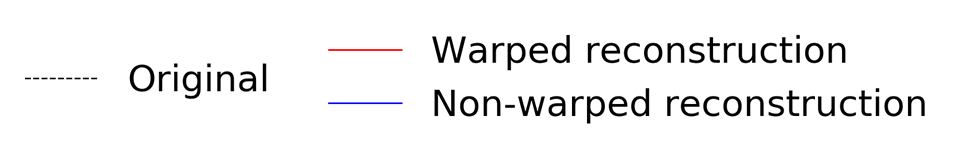
\includegraphics[width=\linewidth]{img/results_techniqueLegend.png}
	\end{subfigure} \\
	\begin{subfigure}[t]{0.32\textwidth}
		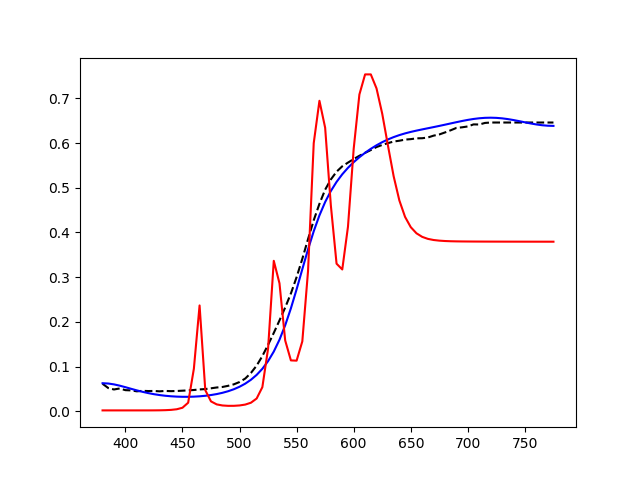
\includegraphics[width=\linewidth]{img/results_warping_orange.png}
		\caption{``orange'' patch}
		\label{fig:warping_alp_neutral50}
	\end{subfigure} \hspace{0.1em}
	\begin{subfigure}[t]{0.32\textwidth}
	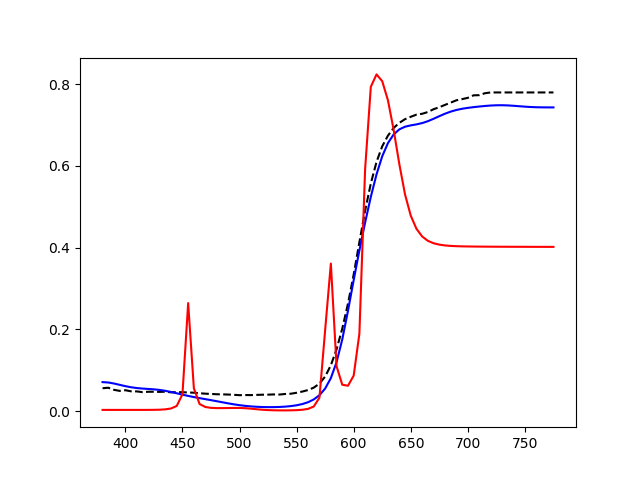
\includegraphics[width=\linewidth]{img/results_warping_red.png}
	\caption{``red'' patch}
	\label{fig:warping_alp_red}
	\end{subfigure} \hspace{0.1em}
	\begin{subfigure}[t]{0.32\textwidth}
		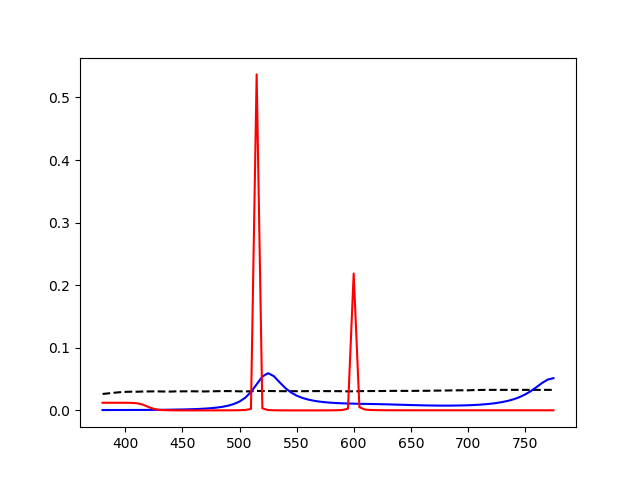
\includegraphics[width=\linewidth]{img/results_warping_black.png}
		\caption{``black'' patch}
		\label{fig:warping_alp_black}
	\end{subfigure}
	\caption{Failure of warping when fitting atlas lattice points, shown on patches from the Macbeth Color Chart}
	\label{fig:warping_atlasLatticePoints}
\end{figure}

For the regular lattice points, we present a similar comparison in~\cref{fig:warping_regularPoints}, where we seed cubes of different sizes with distinct atlases and analyze the spectra at specific points. Not warping the signal is superior to warping even in this case, as it creates smoother spectra with less sharp edges. 

As we eventually decide on using only 3 coefficients per regular lattice points (see~\cref{ssec:noOfMoments}), and for that purpose, even warping works reasonably well, we do not need necessarily to account for regular lattice points when choosing whether to warp the signal. However, regardless, all the presented evidence points to the superiority of non-warping.

\begin{figure}[t]
	\centering
	\captionsetup[subfigure]{font=footnotesize,labelfont=footnotesize}
	\captionsetup[subfigure]{justification=centering}
	\begin{subfigure}[t]{0.38\textwidth}
		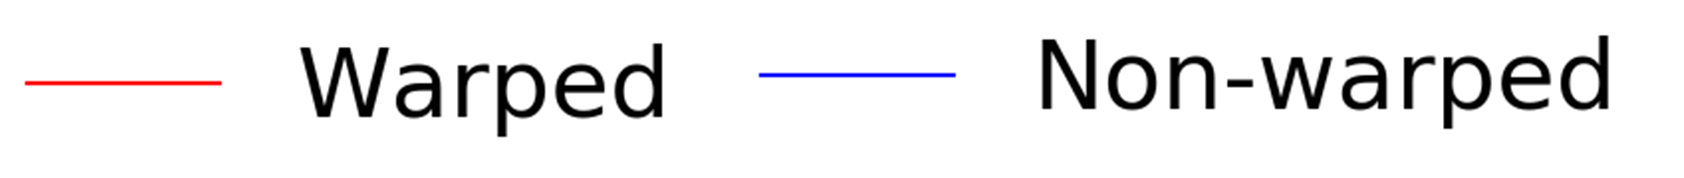
\includegraphics[width=\linewidth]{img/resultsTechniqueOpt_legend.png}
	\end{subfigure} \\
	\begin{subfigure}[t]{0.31\textwidth}
		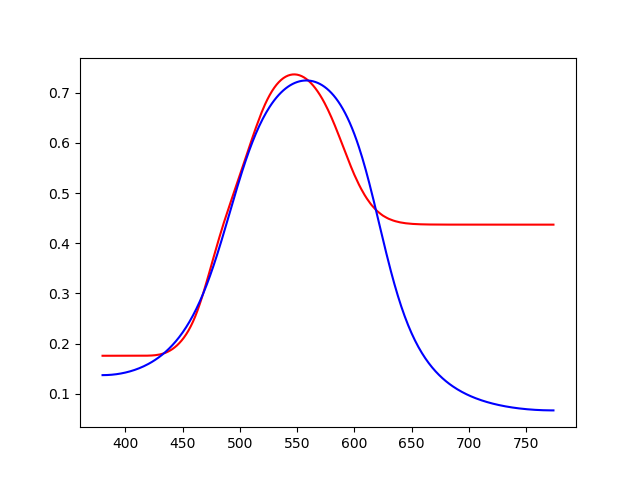
\includegraphics[width=\linewidth]{img/resultsTechniqueOpt_m3_cd64.png}
		\caption{$c=3, cd=64$,\\$RGB=(222.6, 230.7, 230.7)$,\\initial atlas = Macbeth Color Chart}
		\label{fig:warping_regularPointst_m3_cd64}
	\end{subfigure}
	\begin{subfigure}[t]{0.31\textwidth}
		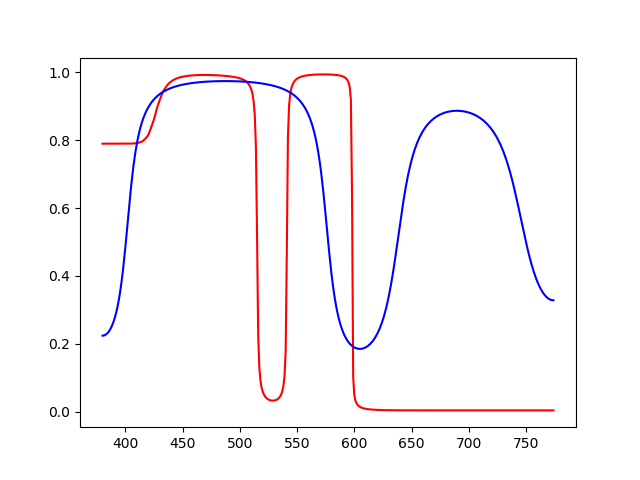
\includegraphics[width=\linewidth]{img/resultsTechniqueOpt_m5_cd32.png}
		\caption{$c=5, cd=32$,\\$RGB=(82.26, 172.74, 255)$,\\initial atlas = Page 14 from Munsell Book of Color}
		\label{fig:warping_regularPoints_m5_cd32}
	\end{subfigure}
	\begin{subfigure}[t]{0.31\textwidth}
		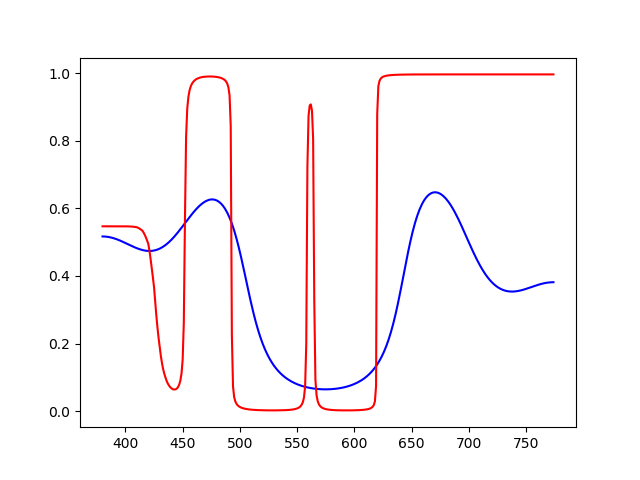
\includegraphics[width=\linewidth]{img/resultsTechniqueOpt_m7_cd16.png}
		\caption{$c=7, cd=16$,\\$RGB=(102, 17, 153)$,\\ fitted from middle}
		\label{fig:warping_regularPoints_m7_cd16}
	\end{subfigure} 
	\caption{Comparison of warping and non-warping when used for fitting regular atlas entries. Note that the figures are illustrative, as they were created with an older version of the cube and therefore may not correspond to the current results.}
	\label{fig:warping_regularPoints}
\end{figure}

To justify the failures of warping, we first analyze its behavior during round-trips in comparison to that of not warping. In~\cref{fig:resultsWarping}, we present a few such examples on different curves with different number of coefficients. We can clearly observe the behavior for which warping was designated --- while the slight waves in the middle of the curve (at around 550nm) are reconstructed almost perfectly, the edges of the curve (i.e. the part of the curve leading up to 450nm and from 650nm) are flat and attain constant values.

If warping the signal, the optimizer therefore has very little influence on the edges of the curve, and therefore opts for optimizing only its middle, which might result in amplifying the already created sinusoidal-shapes.

By not warping the signal, on the other hand, the optimizer focuses on the spectra as a whole and is therefore less prone to spiky artifacts.

Therefore, we conclude that mirroring, but not warping the signal is the optimal approach for our purposes.

\begin{figure}[t]
	\centering
	\captionsetup[subfigure]{font=footnotesize,labelfont=footnotesize}
	\captionsetup[subfigure]{justification=centering}
	\begin{subfigure}[t]{0.60\textwidth}
		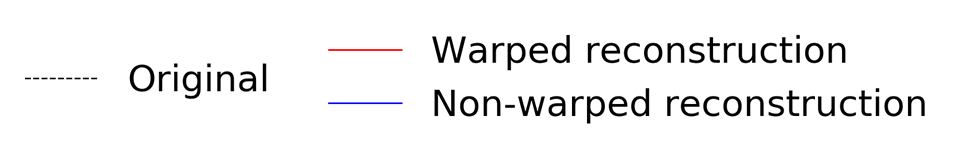
\includegraphics[width=\linewidth]{img/results_techniqueLegend.png}
	\end{subfigure} \\
	\begin{subfigure}[t]{0.45\textwidth}
		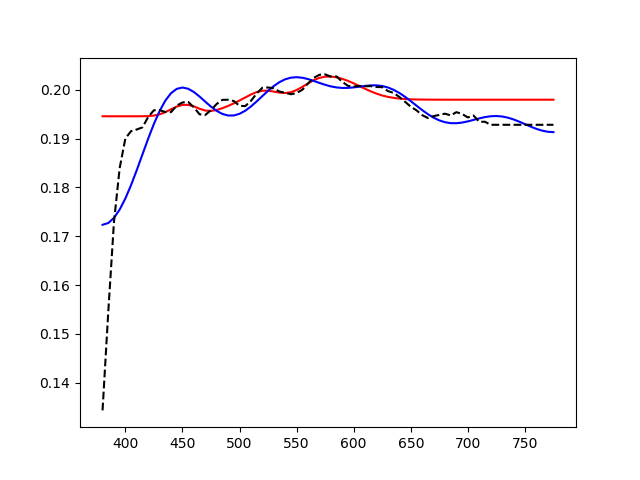
\includegraphics[width=\linewidth]{img/results_techniqueNeutral5.png}
		\caption{``neutral 5'' patch, $c = 9$}
		\label{fig:resultsWarping_neutral5}
	\end{subfigure} \hspace{0.1em}
	\begin{subfigure}[t]{0.45\textwidth}
		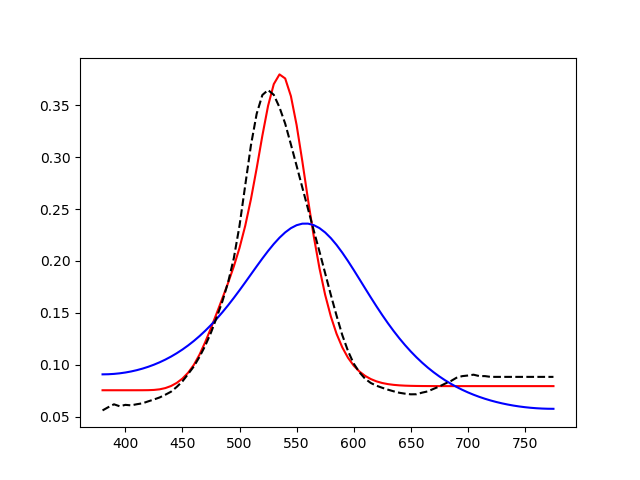
\includegraphics[width=\linewidth]{img/results_techniqueGreen.png}
		\caption{``green'' patch, $c = 3$}
		\label{fig:resultsWarping_green}
	\end{subfigure} \hspace{0.1em}
	\vspace{0.5em}\\
	\begin{subfigure}[t]{0.45\textwidth}
		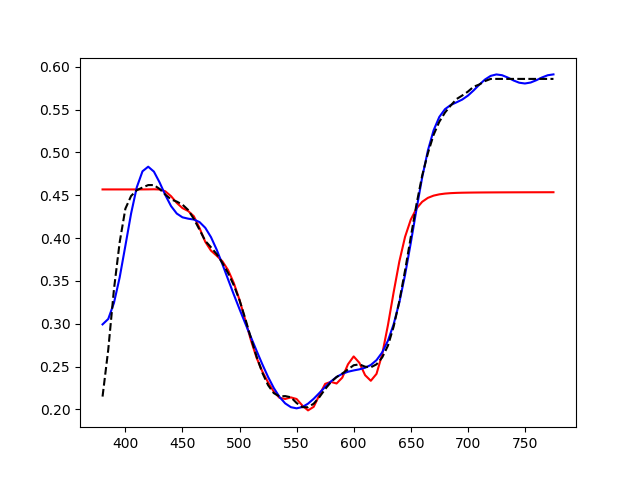
\includegraphics[width=\linewidth]{img/results_techniqueBlueFlower.png}
		\caption{``blue flower'' patch, $c = 16$}
		\label{fig:resultsWarping_blueFlower}
	\end{subfigure} \hspace{0.1em}
	\begin{subfigure}[t]{0.45\textwidth}
		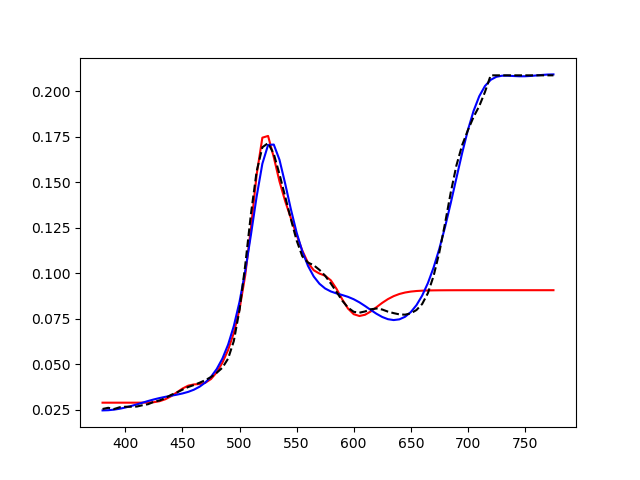
\includegraphics[width=\linewidth]{img/results_techniqueFoliage.png}
		\caption{``foliage'' patch, $c = 12$}
		\label{fig:resultsWarping_foliage}
	\end{subfigure}
	\caption{Comparison between the warped and non-warped reconstructed signal shown on multiple patches of the Munsell Book of Colours}
	\label{fig:resultsWarping}
\end{figure}

\subsection{Number of moments} \label{ssec:noOfMoments}

Another important parameter to determine is the number of moments (or coefficients) with which to store spectra at both atlas lattice points and regular lattice points.

We start by analyzing the atlas lattice points. Specifically, we focus on the number of coefficients with which to store atlas entries in step one ref of our implementation, as those are the coefficients that are then used as prior for atlas lattice points. We wish for these coefficients to reconstruct spectra that resemble the original ones as much as possible, so as to avoid color errors under arbitrary illuminants.

\begin{figure}[t!]
	\centering
	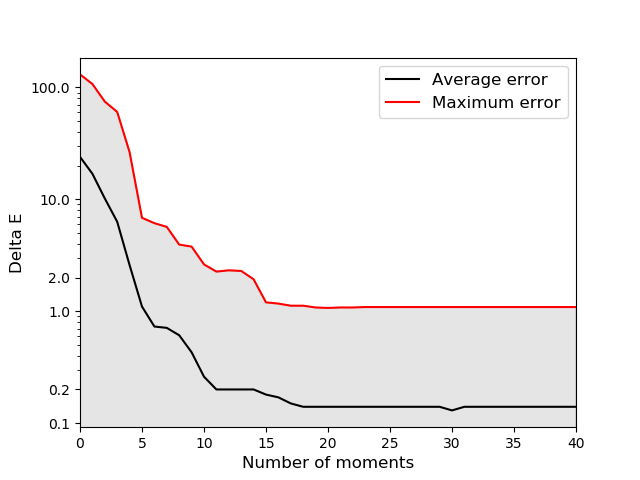
\includegraphics[width=0.6\linewidth]{img/results_noOfMoments_deltaE.png}
	\caption{An}
	\label{fig:results_noOfMoments_deltaE}
\end{figure}

By observing~\cref{fig:results_noOfMoments_deltaE}, we see that the Delta E error obtained by round-trips under the CIE illuminants stabilizes at $m=20$, i.e. $c=21$. As the curve precision does not worsen by adding more coefficients to the representation, storing all atlas entries with 21 coefficients might seem to be the optimal solution. However, as already mentioned in ref, it is beneficial for the performance of the optimizer (both from the viewpoint of the resulting curve's shape and the time complexity) to use as little coefficients as possible.

Therefore, we decide to store each spectrum with only the necessary number of coefficients. For each atlas entry, we obtain them iteratively --- starting from $c=4$, we check whether the coefficient count is sufficient, and, if not, we increase it and move on to the next iteration, repeating this process up to $m=24$.

We determine the sufficiency of a coefficient representation by picking one of the most error-prone illuminants and determining the round-trip error under said illuminant. If the error falls below a certain, pre-defined threshold, we declare the representation sufficient.

We pick the illuminant used for these purposes from the list of the CIE illuminants (excluding the E and D73 illuminants, as these are not yet supported in ART, where we run the experiments). First, we compute the average number of required coefficients to achieve a specific error for each of them. By the assumption that these results give us a rough approximation of the average error, we conclude that the illuminant with the highest coefficient count is the most error-prone.

We present the results of our experiment in~\cref{table:sufficientCoefficientIlluminants}. We use an error of $\Delta E_{ab}^*=0.1$ due to the coefficient count variability under it, but any other would give similar results in terms of the order of the illuminants' coefficient counts.

Since the FL11 illuminant requires the highest number of coefficients, we use it for our purposes, and move on to examining the optimal threshold.

Surprisingly, utilizing the Delta E error in our iterative process of acquiring coefficients did not provide as satisfactory results as expected --- the entries represented with high number of coefficients ($c \ge 20$) were often unnecessarily accurate, while the entries represented with low number of coefficients ($c \le 10$) often lacked precision. Therefore, we decided to compute the error as an  absolute difference over all three RGB components, which outperformed both the Delta E error and even the Euclidean error in the RGB space (which was prone to similar, but less noticeable, behavior than the Delta E error). We set the threshold to $0.1$ for an RGB range of $(0,255)$, as we found it to perform well when tested for the actual uplifting. 

Although we attribute the failure of Delta E to its non-linearity, we have not yet obtained evidence as to support this claim.

Our approach for determining the sufficiency of coefficients is definitely not flawless. Firstly, neither the threshold, nor the computation of the error have been properly examined, which implies that there may be other, more suitable options. Secondly, since we examine only 18 CIE illuminants, there is a high chance that other, more error-prone, exist.

Even the assumption that the average coefficient counts determine the worst-performing illuminant falls short. As we have come across multiple atlas entries that attain the highest color error under an illuminant other than FL11, checking whether the error satisfies the threshold for all illuminants might be a more effective approach.

Furthermore, even if we were to perfect our method, there exist a lot more, vastly different approaches that might be used. However, their exploration and analysis is not within the scope of this thesis, and, as our method produces reasonable results, we leave it for future work.

\begin{table}[t]
	\newcolumntype{?}{!{\vrule width 1.5pt}}
	\centering
	\begin{tabular}{c|c?c|c?c|c}
		\hline
		\rule{0pt}{5ex}
		Illuminant & \makecell{Average\\error} & Illuminant & \makecell{Average\\error}&Illuminant & \makecell{Average\\error}\\ 
		\hline
		\rule{0pt}{3ex}
		A & 14.8 & F & 12.91 & F7 & 12.55 \\ 
		B & 5.19 & F2 & 13.01 & F8 & 12.01 \\ 
		C & 16.11 & F3 & 12.93 & F9 & 12.09 \\ 
		D50 & 15.56 & F4 & 12.98 & F10 & 16.24 \\ 
		D65 & 15.64 & F5 & 12.95 & F11 & 16.46 \\ 
		D75 & 15.76 & F6 & 13.08 & F12 & 16.30 \\ 
		\hline
	\end{tabular}
	\caption{The average number of coefficients needed to achieve a round-trip error of $\Delta E_{ab}^* = 0.1$ for different CIE illuminants}
	\label{table:sufficientCoefficientIlluminants}
\end{table}

Finding the sufficient coefficient count for regular lattice points is a lot more straightforward than for the atlas lattice points. We remind that, in order to avoid interpolation-caused artifacts, we require their spectra to be smooth. This property is especially important if two significantly different, spiky atlas entries are fitted in voxels close to each other. Propagating their original shapes during the cube fitting process would, under a different illuminant, create a noticeable border between the two colors, which is undesired. Rather, we want to see smooth gradients.

Figure~\cref{fig:warping_regularPoints} already suggests that using less coefficients might benefit our smoothness requirement. We put this theory to test by comparing spectra of regular lattice points fitted with a different number of coefficients in cubes of otherwise identical parameters. We present some of the results in~\cref{fig:noOfMoments_regularPoints}.

\begin{figure}[t]
	\centering
	\captionsetup[subfigure]{font=footnotesize,labelfont=footnotesize}
	\captionsetup[subfigure]{justification=centering}
	\begin{subfigure}[t]{0.60\textwidth}
		
\includegraphics[width=\linewidth]{img/results_noOfMoments_regularPts_legend.png}
	\end{subfigure} \\
	\begin{subfigure}[t]{0.45\textwidth}
		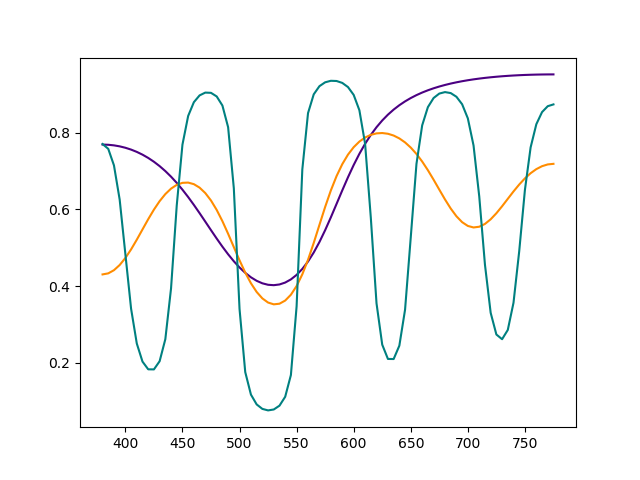
\includegraphics[width=\linewidth]{img/results_noOfMoments_regularPts_1.png}
		\caption{$RGB=(222.1, 106.9, 164.5)$,\\ fitting round $= 8/17$}
	\end{subfigure}
	\begin{subfigure}[t]{0.45\textwidth}
		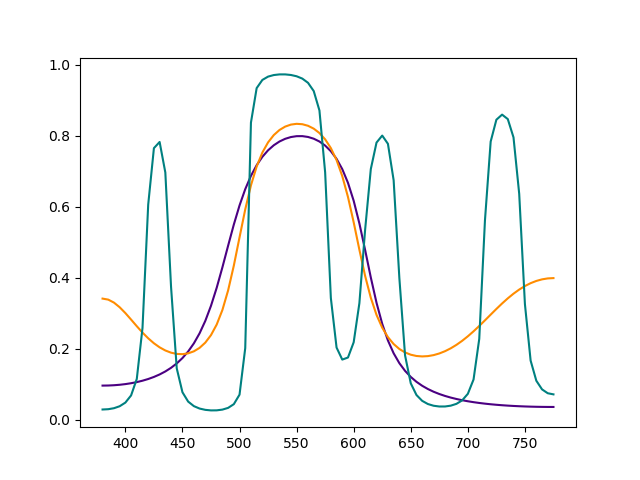
\includegraphics[width=\linewidth]{img/results_noOfMoments_regularPts_2.png}
		\caption{$RGB=(98.7, 205.6, 41.1)$,\\ fitting round $= 9/17$}
	\end{subfigure} 
	\caption{Comparison of spectra at regular lattice points when fitting . Cube }
	\label{fig:noOfMoments_regularPoints}
\end{figure}

Our assumptions have proven to be correct. By using less coefficients, we limit the optimizer's ability to reconstruct complicated spectra, therefore forcing it to create smooth, simple shapes. Specifically, we decide on using 3 coefficients --- as their shapes are sufficient, using more is unnecessary, however 2 were unable to recreate shapes and often ended up being constant, straight lines.

Additional benefit of using only 3 coefficients per regular lattice point is the lower run-time of cube fitting in comparison to higher number of coefficients, as well as less optimizer failures and therefore no need for invocation of heuristic improvements.

\subsection{Cost functions} \label{ssec:costFunctions}

In addition to the moment storage technique, another thing greatly affecting the performance of the fitting are the cost functions of optimizer.

For the fitting of the sigmoids, Borgtool uses three cost functions, or \emph{residuals}, each of them specifying the absolute color difference in one axis of the RGB cube. Such an approach outperforms both the Euclidean color distance and even the Delta E difference --- the higher the number of meaningful residuals, the more information about the coefficients' behavior can the optimizer deduce, which, in turn, results in faster and more precise convergence to global optimum.

As this approach performs rather decently in terms of both time complexity and the obtained results for the sigmoids, we try it out for the purposes of our optimization as well. 

In case of fitting of the regular lattice points (see~\cref{ssec:cubeFitting}), which requires the manipulation of 3 coefficients, the obtained results are satisfactory, both for the fitting in the second round and in the latter rounds (see~\cref{fig:costFunctionsRegularFitting}). The resulting curves are smooth, which suits the interpolation process during rendering, they evaluate to the desired RGB values, and the run-time is even better than for the sigmoids. Therefore, we utilize this approach for the regular lattice points.

\begin{figure}[t]
	\centering
	\begin{subfigure}[t]{0.4\textwidth}
		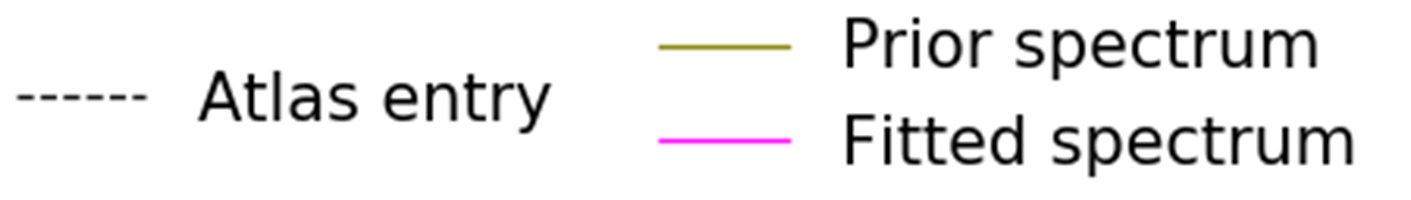
\includegraphics[width=\linewidth]{img/cost_functions_regular_legend.png}
	\end{subfigure} \\
	\begin{subfigure}[t]{0.45\textwidth}
	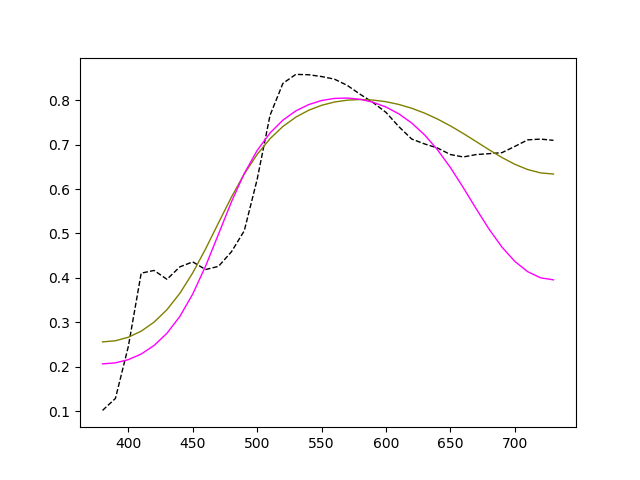
\includegraphics[width=\linewidth]{img/cost_functions_regular_round2.png}
	\caption{Fitting in the second round, i.e. the prior coefficients are the result of ``recomputation'' of the fitted coefficients of an atlas lattice point}
	\label{fig:costFunctionsRegularRound2}
	\end{subfigure} \hspace{0.1em}
	\begin{subfigure}[t]{0.45\textwidth}
		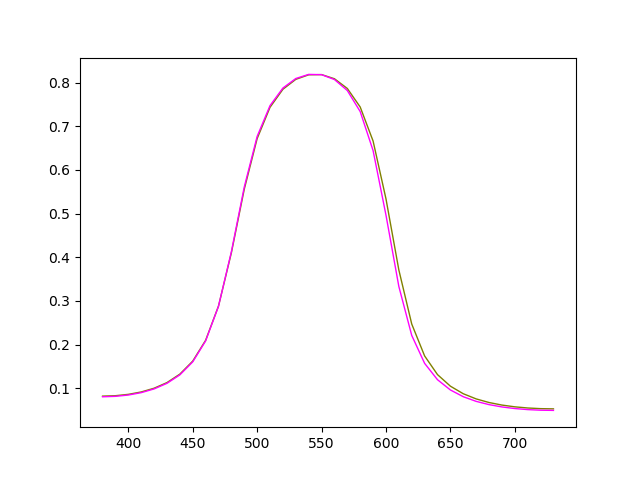
\includegraphics[width=\linewidth,height=0.2\textheight]{img/cost_functions_regular_round8.png}
		\caption{Fitting in round 8/20, where the prior spectrum is that of a regular lattice point}
		\label{fig:costFunctionsRegularRound8}
	\end{subfigure} 
	\caption{Fitting of regular lattice points with 3 cost functions specifying the RGB difference}
	\label{fig:costFunctionsRegularFitting}
\end{figure}

However, when fitting the atlas lattice points (see~\cref{ssec:startingPointsFitting}), the fact that the cost functions do not take the resulting shape of the spectra into account in any way works to our disadvantage. We show an example of this in~\cref{fig:resultsCostFunctions} on the magenta plot, which demonstrates the performance of fitting of atlas lattice points with RGB cost functions only. Although it terminates as successful (as the RGB of the resulting curve is within the fitting threshold of the target RGB), the reflectance curve takes on a sinusoidal shape with a rather high amplitude, therefore losing resemblance to the original curve. This is due to definition of coefficients, which are, in their nature, Fourier coefficients, and are therefore prone to exhibiting this type of behavior. This is mainly perceivable when the color distance $d$ between the atlas entry and atlas lattice point is rather high, as it gives the optimizer enough room to make visible changes in the shape of the reconstructed spectrum before converging below the fitting threshold.
 
Note that we compare the fitted spectra not with the original atlas spectra, but with the spectra that is reconstructed from the original's coefficients to keep track of the optimizer's ability to mimic its input.

\begin{figure}[t]
	\centering
	\captionsetup[subfigure]{font=footnotesize,labelfont=footnotesize}
	\captionsetup[subfigure]{justification=centering}
	\begin{subfigure}[t]{0.70\textwidth}
		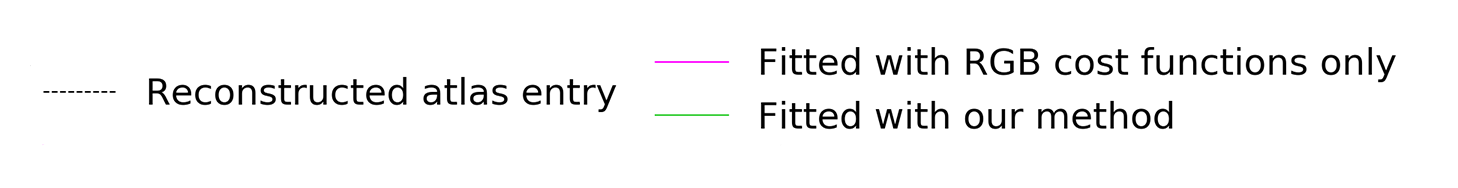
\includegraphics[width=\linewidth]{img/results_costFunctions_legend.png}
	\end{subfigure} \\
	\begin{subfigure}[t]{0.45\textwidth}
		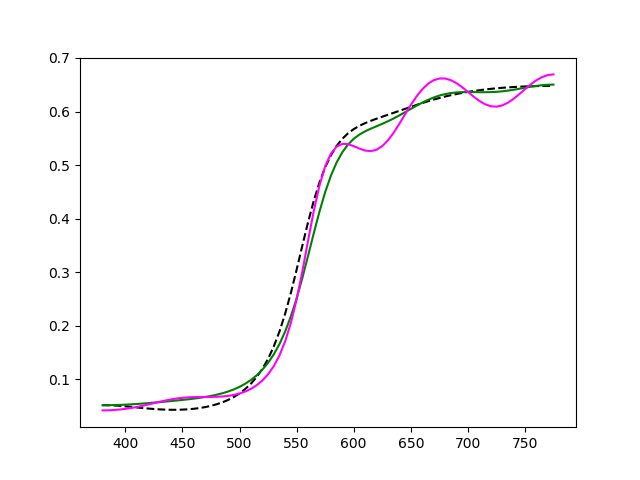
\includegraphics[width=\linewidth]{img/results_costFunctions_orange.png}
		\caption{``orange'' patch of the MCC, $c = 8$, $d = 11.84$}
		\label{fig:resultsCostFunctions_orange}
	\end{subfigure} \hspace{0.1em}
	\begin{subfigure}[t]{0.45\textwidth}
		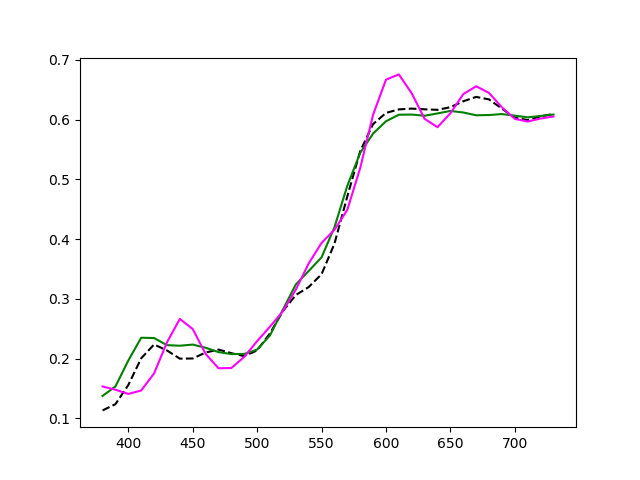
\includegraphics[width=\linewidth]{img/results_costFunctions_mcb0706.png}
		\caption{5YR 7/6 patch of the MBC, $c = 14$, $d = 5.85$}
		\label{fig:resultsCostFunctions_mcb0706}
	\end{subfigure} 
	\vspace{0.5em}\\
	\begin{subfigure}[t]{0.45\textwidth}
		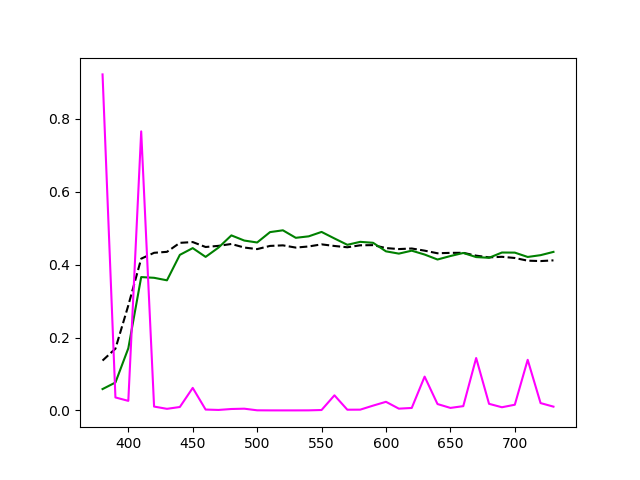
\includegraphics[width=\linewidth]{img/results_costFunctions_mcb0725.png}
		\caption{N 7.25 patch of the MBC, $c = 20$, $d = 12.67$}
		\label{fig:resultsCostFunctions_mcb0725}
	\end{subfigure} \hspace{0.1em}
	\begin{subfigure}[t]{0.45\textwidth}
		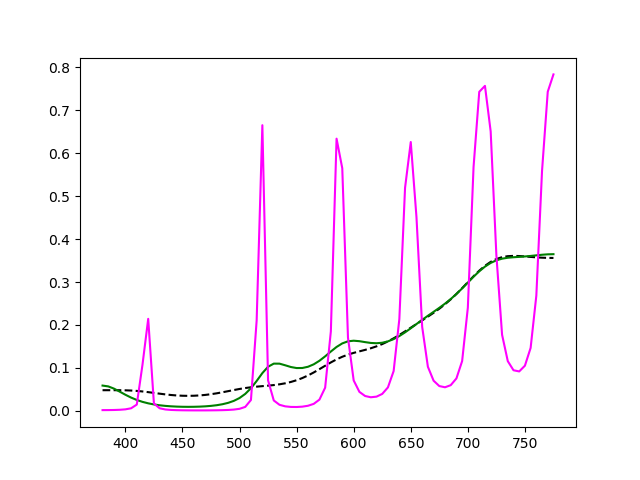
\includegraphics[width=\linewidth]{img/results_costFunctions_darkskin.png}
		\caption{``dark skin'' patch of the MCC, $c = 12$, $d = 11.55$}
		\label{fig:resultsCostFunctions_darkskin}
	\end{subfigure}
	\caption{Comparison between the RGB cost functions and our method for fitting atlas lattice points}
	\label{fig:resultsCostFunctions}
\end{figure}

We therefore conclude that we must incorporate the requirement of curve shape similarity into our cost functions. Following, we review the cost functions that we tried along with their performance.

Firstly, we implemented an approach similar to that for determining the number of coefficients with which to store atlas entries (see ref), i.e. we utilized the color error under a fluorescent illuminant (specifically, FL11). We defined three additional cost functions, each specifying the difference between the original and the reconstructed curve's RGB under the FL11 illuminant in one of the axes. If their values fell below a specific threshold, we terminated the fitting process as successful, if not, we increased the threshold and tried again.

Although this approach was successful on average (the average threshold was around $t = 0.025$), on occasion, the threshold often needed to be increased to values so high that it became obsolete. Using only one error, either the Euclidean distance or the Delta E error, caused similar issues.

Therefore, we decided to focus on the actual distance between the two curves. Our first attempt consisted of defining one residual per wavelength sample specifying the absolute distance between the two spectra at said wavelength (as the least square error proved to perform worse). We examined the performance of both around 360 residuals (i.e. 1nm increment between samples) and 36 residuals (10nm increment, as defined in most color atlases) when used alongside the 3 already defined RGB residuals. For $c \le 9$, both of these options performed reasonably well. When fitting more coefficients, the sufficient threshold was, on average, around $t = 0.0096$, both before and after the introduction of our improvement of optimizing only first 4 coefficients, and although its maximum ended up being $t = 0.23$, overall, this method outperformed the previous one.

As we suspected that the failures were caused by the abundance of cost functions, we summed up their values and saved them into a single residual, which, when divided by the number of spectral samples, represented the average error per sample.

As the importance of curve samples in terms of proper color reconstruction is mainly placed on their middle (at around 550nm), we attempted to add a heuristic-based weighting factor in an effort to focus on minimizing the distance between the two curve there. However, we did not succeed in improving our results, and we therefore dropped the experiment and examined the performance without weighting the values.

Such an approach substantially outperformed the previous ones, and even more after we decided to specify the absolute error rather than the least square error. The average error ended up being only about $d = $, and, of yet, no entry requiring $d > $ has been encountered. Therefore, we concluded that the optimal solution to our problem is to set 4 residuals, 3 specifying the RGB difference, and 1 specifying the average distance per sample.

We present some of the results achieved with our cost functions on the green plot in~\cref{fig:resultsCostFunctions}, where we compare them to fitting with RGB cost functions only. In~\cref{fig:resultsCostFunctions_mcb0725} and~\cref{fig:resultsCostFunctions_darkskin}, we specifically focus on the most problematic spectra with the highest distance $d$ between the atlas lattice point and the atlas entry.

Although our approach substantially reduces the appearance of sinosidual-like behavior, it does not diminish it completely. It can be observed especially for atlas lattice points with $c > 14$ (see~\cref{fig:resultsCostFunctions_mcb0725}). This is due to the fact that we optimize only the first 4 coefficients, which, in their nature, are prone to creating such patterns.

Another drawback of our approach is the substantially larger time complexity, especially if improvement heuristics need to be applied. By examining the scope of the optimizer and utilizing its options further, or maybe even resorting to a different method of optimization, we might be able to improve upon both the time complexity, and the resulting spectral shape.

However, as the runtime is not the focus of this thesis and as the resulting shapes are satisfactory for the purposes of this these, we focused our efforts elsewhere and leave these improvements for future work.

When fitting other spectral data, the optimizer does not behave as drastically as shown in~\cref{fig:resultsCostFunctions}. On the contrary, many fitted altas entries (such as the ``blue flower'' of the Macbeth Color Checker) resemble their input quite well. However, we must focus on the worst-case scenario as we do not wish to experience any metameric artifacts, not even in one color.

\section{Rendering}

In this section, we present the actual results achieved with our process. The way we do it is that
we spectrally render an image using a set of spectra (we denote this image the original image), use this spectra as seeds for the cube, we create the cube and then use this cube for uplifting the original rendered image. 

The ideal way to do this

heuristics performance, overall runtime of the cube



\begin{figure}[t]
	\centering
	{\sffamily
		\begin{tabular}{cccc}
			Spectral render & Sigmoid uplift & Our uplift
			\vspace{1em} \\
			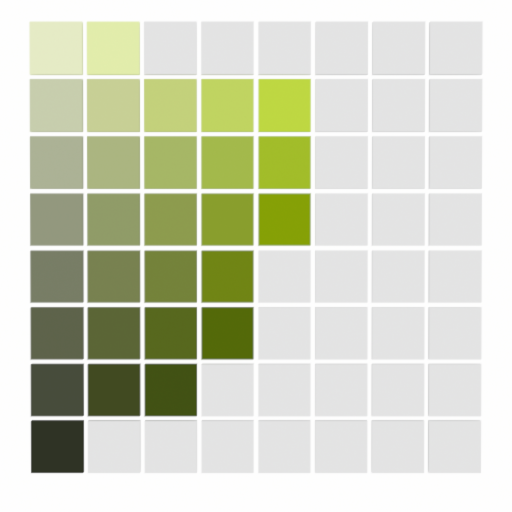
\includegraphics[width=.30\linewidth]{img/results_art_page14_originalD65.png}
			&
			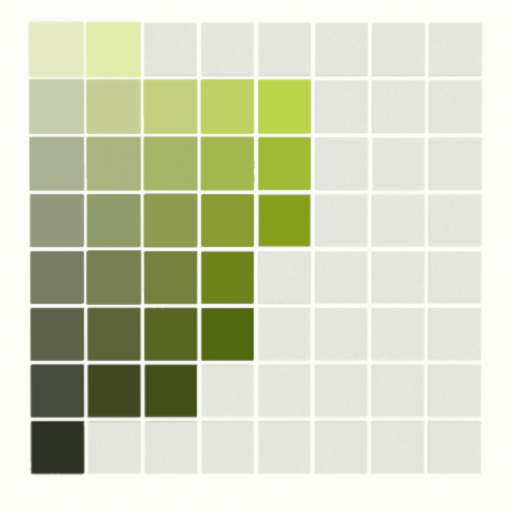
\includegraphics[width=.30\linewidth]{img/results_art_page14_sigmoidD65.png}
			& 
			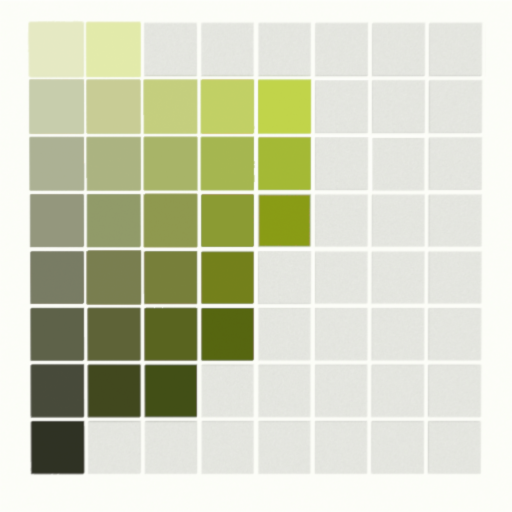
\includegraphics[width=.30\linewidth]{img/results_art_page14_ourD65.png}
			\vspace{1em} \\
			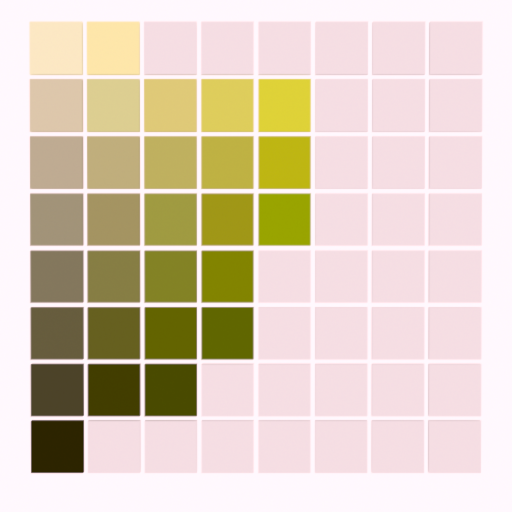
\includegraphics[width=.30\linewidth]{img/results_art_page14_originalFL11.png}
			&
			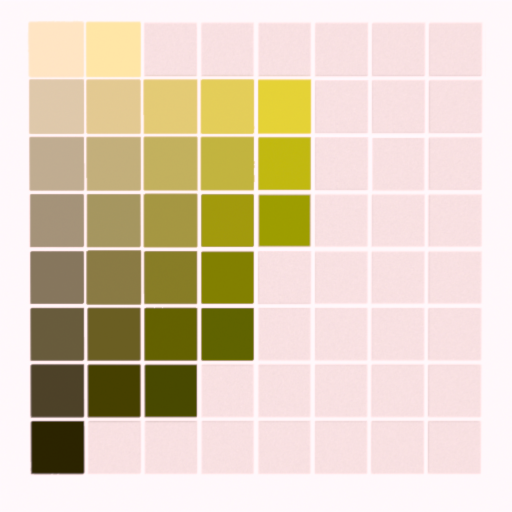
\includegraphics[width=.30\linewidth]{img/results_art_page14_sigmoidFL11.png}
			&
			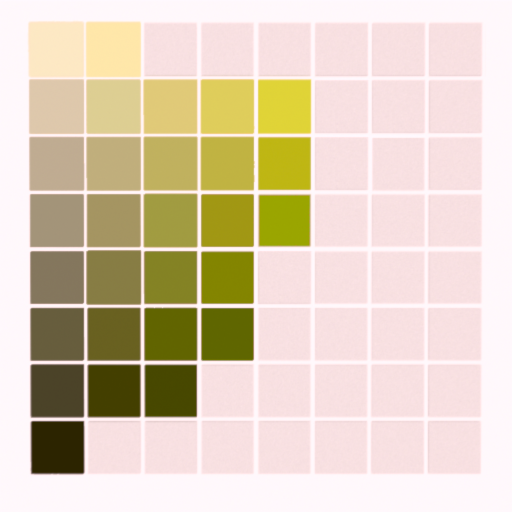
\includegraphics[width=.30\linewidth]{img/results_art_page14_ourFL11.png}
		\end{tabular}
	}
	\caption{Actually rendered with ART.}
	\label{fig:results_art_page14}
\end{figure}


\begin{figure}[t!]
	\centering
	{\sffamily
		\setlength\tabcolsep{0.5pt}
		\begin{tabular}{ccccccc}
			&Original& Uplifted & Difference &\quad Original & Uplifted & Difference
			\vspace{1em} \\ 
			\raisebox{0.4cm}[0pt][0pt]{\parbox[c][0pt][c]{0cm}{\hspace{-1.5em}\rotatebox{90}{Sigmoid}\\[20pt]}\par}
			&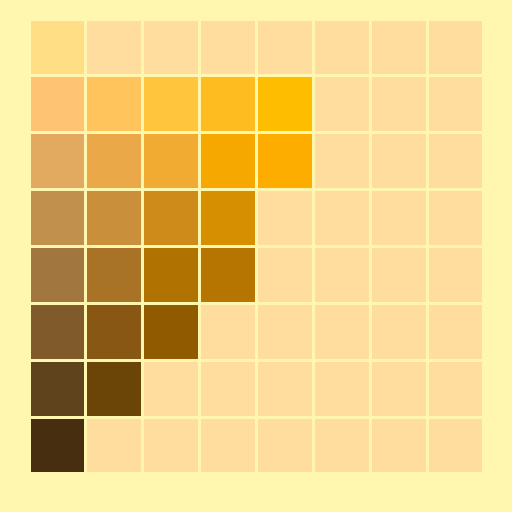
\includegraphics[width=.155\linewidth]{img/results_uplift_page09_originalFL11.png}
			&
			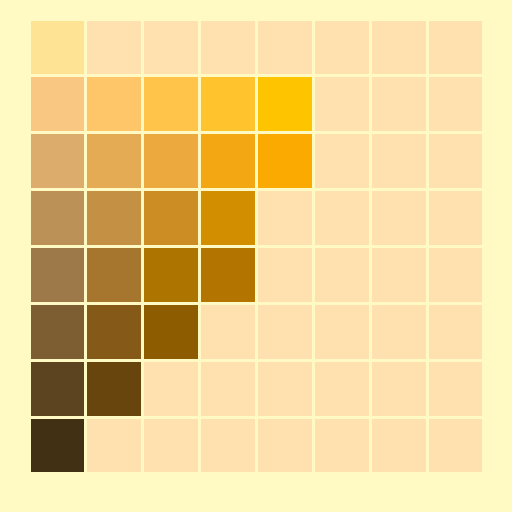
\includegraphics[width=.155\linewidth]{img/results_uplift_page09_sigmoidFL11.png}
			& 
			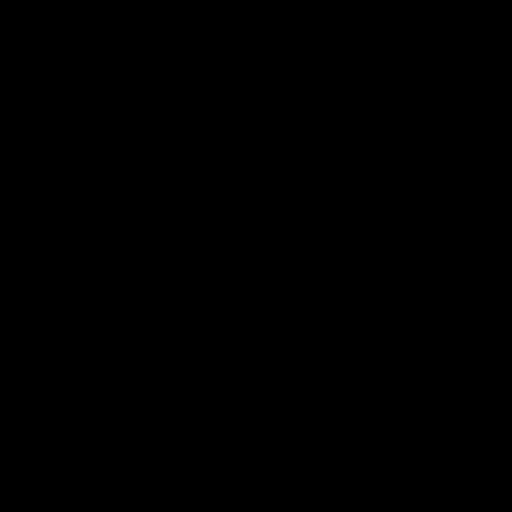
\includegraphics[width=.155\linewidth]{img/toDelete.png}
			&\quad
			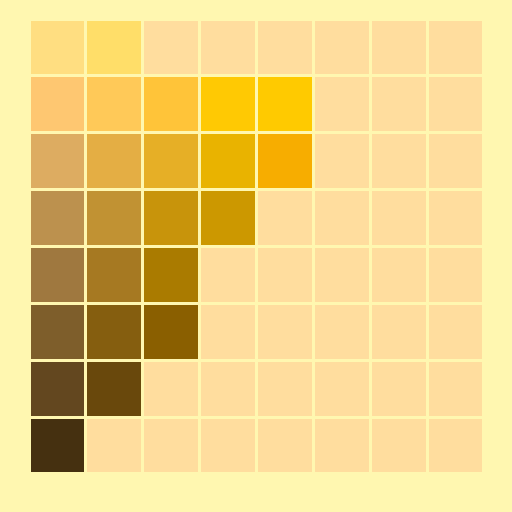
\includegraphics[width=.155\linewidth]{img/results_uplift_page10_originalFL11.png}
			&
			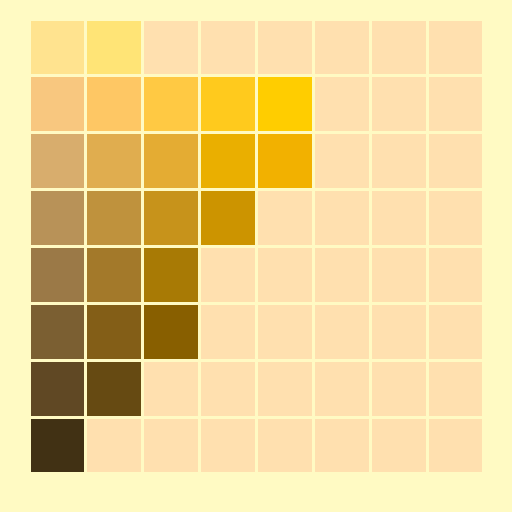
\includegraphics[width=.155\linewidth]{img/results_uplift_page10_sigmoidFL11.png}
			&
			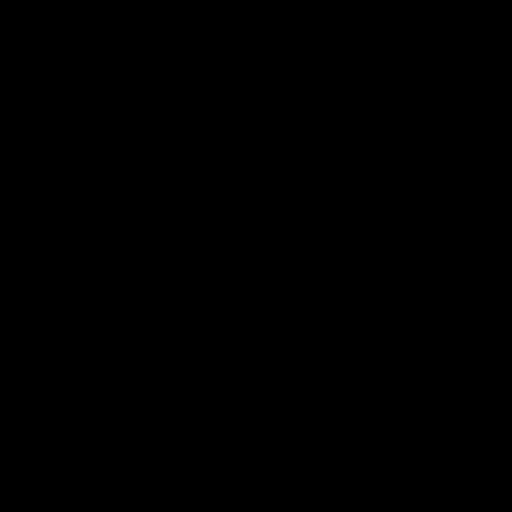
\includegraphics[width=.155\linewidth]{img/toDelete.png}
			\\ \raisebox{0.5cm}[0pt][0pt]{\parbox[c][0pt][c]{0cm}{\hspace{-1.5em}\rotatebox{90}{Our}\\[20pt]}\par}
			&
			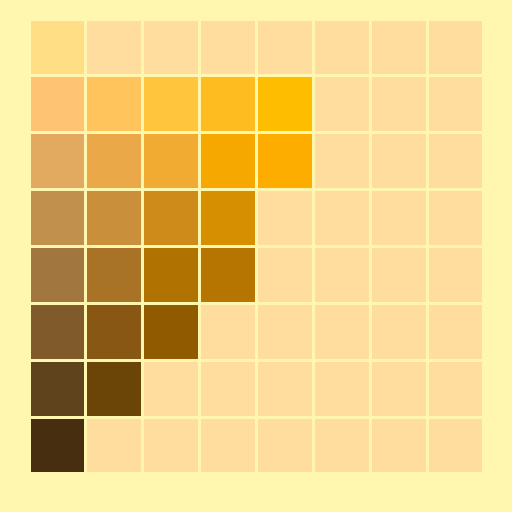
\includegraphics[width=.155\linewidth]{img/results_uplift_page09_originalFL11.png}
			&
			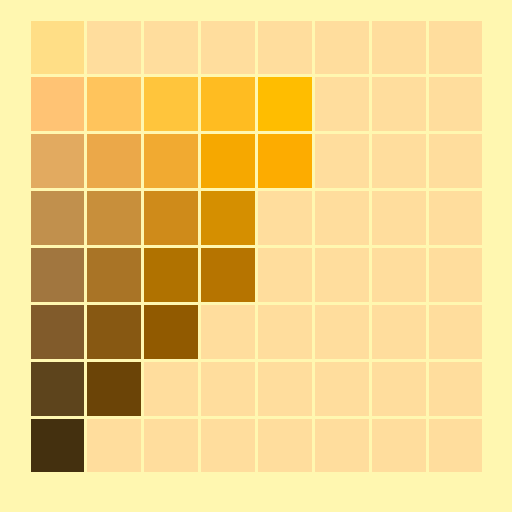
\includegraphics[width=.155\linewidth]{img/results_uplift_page09_ourFL11.png}
			& 
			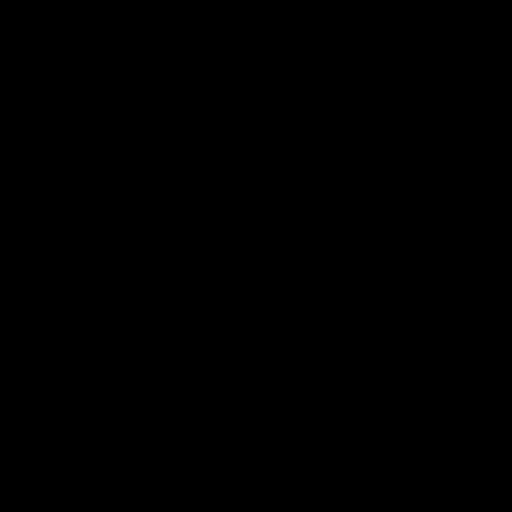
\includegraphics[width=.155\linewidth]{img/toDelete.png}
			&\quad
			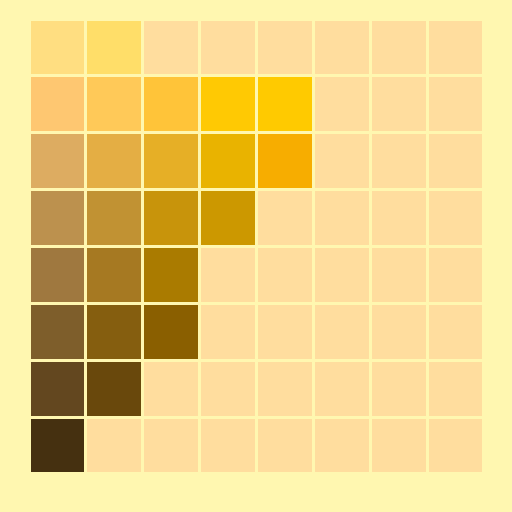
\includegraphics[width=.155\linewidth]{img/results_uplift_page10_originalFL11.png}
			&
			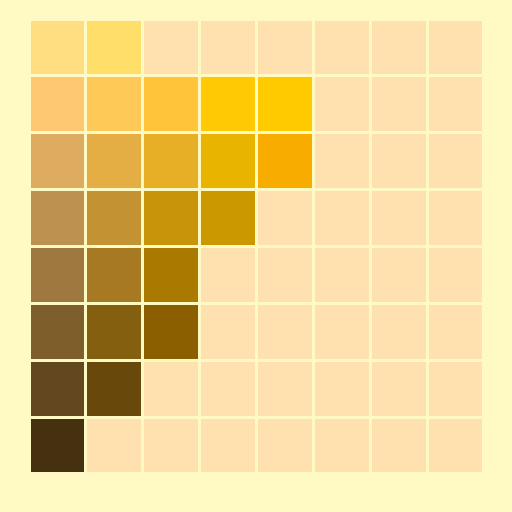
\includegraphics[width=.155\linewidth]{img/results_uplift_page10_ourFL11.png}
			&
			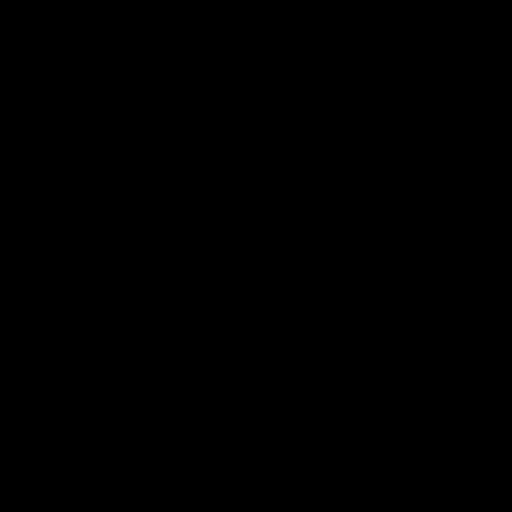
\includegraphics[width=.155\linewidth]{img/toDelete.png}\\
			& & Page 9 & & & Page 10 & \\
			\vspace{0.1em} \\ 
			\raisebox{0.4cm}[0pt][0pt]{\parbox[c][0pt][c]{0cm}{\hspace{-1.5em}\rotatebox{90}{Sigmoid}\\[20pt]}\par}
			&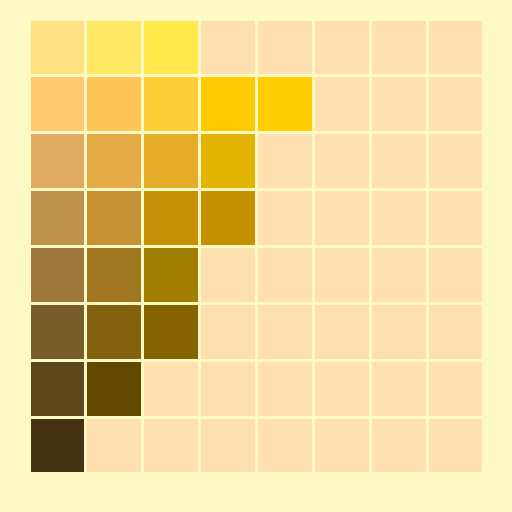
\includegraphics[width=.155\linewidth]{img/results_uplift_page11_originalFL11.png}
			&
			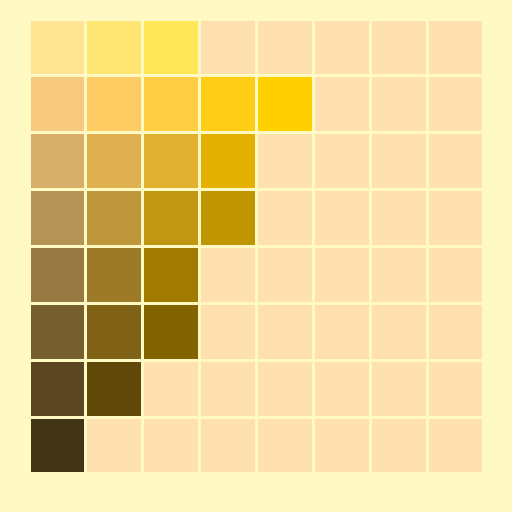
\includegraphics[width=.155\linewidth]{img/results_uplift_page11_sigmoidFL11.png}
			& 
			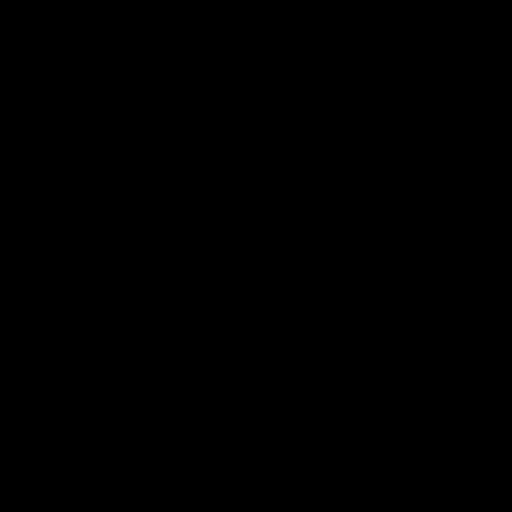
\includegraphics[width=.155\linewidth]{img/toDelete.png}
			&\quad
			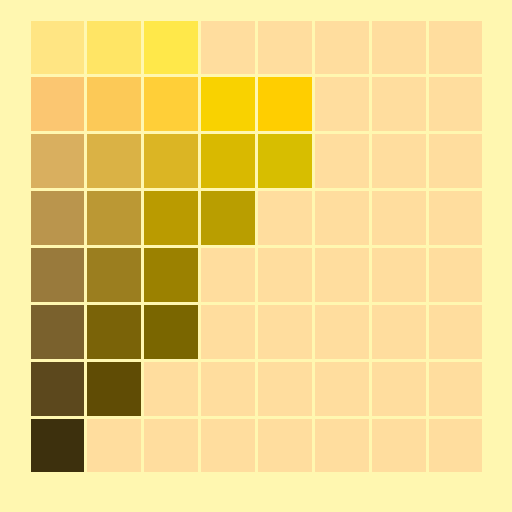
\includegraphics[width=.155\linewidth]{img/results_uplift_page12_originalFL11.png}
			&
			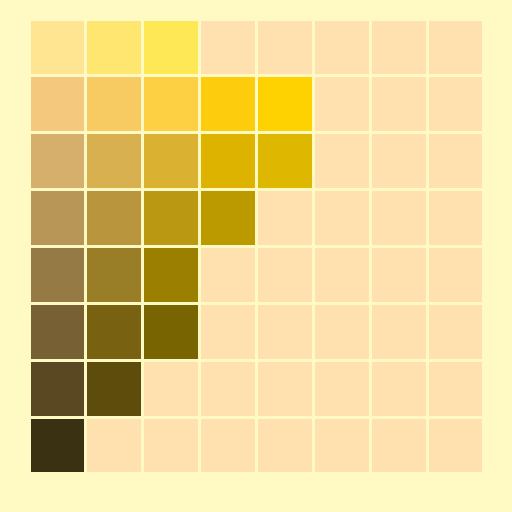
\includegraphics[width=.155\linewidth]{img/results_uplift_page12_sigmoidFL11.png}
			&
			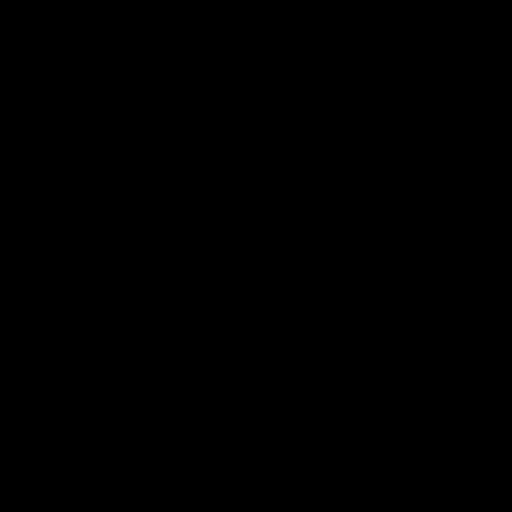
\includegraphics[width=.155\linewidth]{img/toDelete.png}
			\\ \raisebox{0.5cm}[0pt][0pt]{\parbox[c][0pt][c]{0cm}{\hspace{-1.5em}\rotatebox{90}{Our}\\[20pt]}\par}
			&
			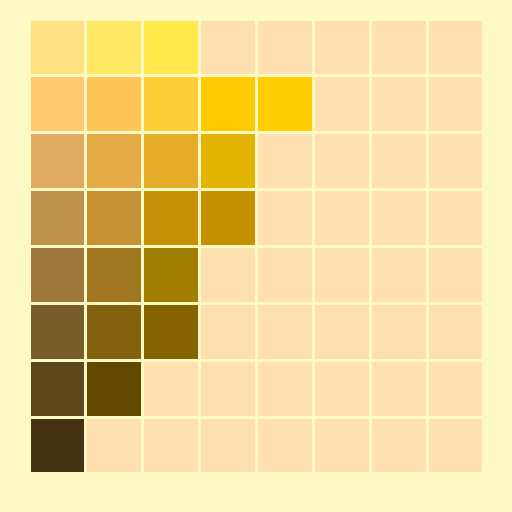
\includegraphics[width=.155\linewidth]{img/results_uplift_page11_originalFL11.png}
			&
			\includegraphics[width=.155\linewidth]{img/results_uplift_page11_ourFL11.png}
			& 
			\includegraphics[width=.155\linewidth]{img/toDelete.png}
			&\quad
			\includegraphics[width=.155\linewidth]{img/results_uplift_page12_originalFL11.png}
			&
			\includegraphics[width=.155\linewidth]{img/results_uplift_page12_ourFL11.png}
			&
			\includegraphics[width=.155\linewidth]{img/toDelete.png}\\
			& & Page 11 & & & Page 12 & \\
			\vspace{0.1em} \\ 
			\raisebox{0.4cm}[0pt][0pt]{\parbox[c][0pt][c]{0cm}{\hspace{-1.5em}\rotatebox{90}{Sigmoid}\\[20pt]}\par}
			&\includegraphics[width=.155\linewidth]{img/results_uplift_page13_originalFL11.png}
			&
			\includegraphics[width=.155\linewidth]{img/results_uplift_page13_sigmoidFL11.png}
			& 
			\includegraphics[width=.155\linewidth]{img/toDelete.png}
			&\quad
			\includegraphics[width=.155\linewidth]{img/results_uplift_page14_originalFL11.png}
			&
			\includegraphics[width=.155\linewidth]{img/results_uplift_page14_sigmoidFL11.png}
			&
			\includegraphics[width=.155\linewidth]{img/toDelete.png}
			\\ \raisebox{0.5cm}[0pt][0pt]{\parbox[c][0pt][c]{0cm}{\hspace{-1.5em}\rotatebox{90}{Our}\\[20pt]}\par}
			&
			\includegraphics[width=.155\linewidth]{img/results_uplift_page13_originalFL11.png}
			&
			\includegraphics[width=.155\linewidth]{img/results_uplift_page13_ourFL11.png}
			& 
			\includegraphics[width=.155\linewidth]{img/toDelete.png}
			&\quad
			\includegraphics[width=.155\linewidth]{img/results_uplift_page14_originalFL11.png}
			&
			\includegraphics[width=.155\linewidth]{img/results_uplift_page14_ourFL11.png}
			&
			\includegraphics[width=.155\linewidth]{img/toDelete.png}\\
			& & Page 13 & & & Page 14 & \\
		\end{tabular}
	}
	\caption{The comparison of the green pages uplift}
	\label{fig:results_uplift_munsell_green_pages}
\end{figure}


 As the variance in the RGB value of the resulting image map is inevitable due to the stochastic nature of the spectral rendering process, - navyse daco s tymto spravit


\begin{figure}[t]
	\centering
	{\sffamily
		\setlength\tabcolsep{0.5pt}
		\begin{tabular}{ccccccc}
			&Original& Uplifted & Difference &\quad Original & Uplifted & Difference
			\vspace{1em} \\ 
			\raisebox{0.4cm}[0pt][0pt]{\parbox[c][0pt][c]{0cm}{\hspace{-1.5em}\rotatebox{90}{Sigmoid}\\[20pt]}\par}
			&\includegraphics[width=.155\linewidth]{img/results_uplift_page04_originalFL3.png}
			&
			\includegraphics[width=.155\linewidth]{img/results_uplift_page04_sigmoidFL3.png}
			& 
			\includegraphics[width=.155\linewidth]{img/toDelete.png}
			&\quad
			\includegraphics[width=.155\linewidth]{img/results_uplift_page10_originalFL11.png}
			&
			\includegraphics[width=.155\linewidth]{img/results_uplift_page10_sigmoidFL11.png}
			&
			\includegraphics[width=.155\linewidth]{img/toDelete.png}
			\\ \raisebox{0.5cm}[0pt][0pt]{\parbox[c][0pt][c]{0cm}{\hspace{-1.5em}\rotatebox{90}{Our}\\[20pt]}\par}
			&
			\includegraphics[width=.155\linewidth]{img/results_uplift_page04_originalFL3.png}
			&
			\includegraphics[width=.155\linewidth]{img/results_uplift_page04_ourFL3.png}
			& 
			\includegraphics[width=.155\linewidth]{img/toDelete.png}
			&\quad
			\includegraphics[width=.155\linewidth]{img/results_uplift_page10_originalFL11.png}
			&
			\includegraphics[width=.155\linewidth]{img/results_uplift_page10_ourFL11.png}
			&
			\includegraphics[width=.155\linewidth]{img/toDelete.png}\\
			& & Page 4; FL 3 & & & Page 24; D65 & \\
			\vspace{0.1em} \\ 
			\raisebox{0.4cm}[0pt][0pt]{\parbox[c][0pt][c]{0cm}{\hspace{-1.5em}\rotatebox{90}{Sigmoid}\\[20pt]}\par}
			&\includegraphics[width=.155\linewidth]{img/results_uplift_page11_originalFL11.png}
			&
			\includegraphics[width=.155\linewidth]{img/results_uplift_page11_sigmoidFL11.png}
			& 
			\includegraphics[width=.155\linewidth]{img/toDelete.png}
			&\quad
			\includegraphics[width=.155\linewidth]{img/results_uplift_page35_originalD50.png}
			&
			\includegraphics[width=.155\linewidth]{img/results_uplift_page35_sigmoidD50.png}
			&
			\includegraphics[width=.155\linewidth]{img/toDelete.png}
			\\ \raisebox{0.5cm}[0pt][0pt]{\parbox[c][0pt][c]{0cm}{\hspace{-1.5em}\rotatebox{90}{Our}\\[20pt]}\par}
			&
			\includegraphics[width=.155\linewidth]{img/results_uplift_page11_originalFL11.png}
			&
			\includegraphics[width=.155\linewidth]{img/results_uplift_page11_ourFL11.png}
			& 
			\includegraphics[width=.155\linewidth]{img/toDelete.png}
			&\quad
			\includegraphics[width=.155\linewidth]{img/results_uplift_page35_originalD50.png}
			&
			\includegraphics[width=.155\linewidth]{img/results_uplift_page35_ourD50.png}
			&
			\includegraphics[width=.155\linewidth]{img/toDelete.png}\\
			& & Page 29, FL 7 & & & Page 35, D50 & \\
		\end{tabular}
	}
	\caption{Comparison of other pages}
	\label{fig:results_uplift_munsell_other}
\end{figure}

- which technique gives the best results (metamerism results)


Also mention that it is multi-threaded and performance is not really a priority - the cube has to be created only once and then can be reused as much as the artists need.
